% Section content template for individual Educative lessons
% This file contains the actual content for a specific section
% Generated from Educative API section content

% Section: Class Diagram for the Online Stock Brokerage System
% Section ID: 4575406147764224
% Section Slug: class-diagram-for-the-online-stock-brokerage-system
% Generated: 2025-12-14T12:54:27.217028

In this lesson, we'll identify and design the classes, abstract classes, and interfaces based on the requirements we have previously gathered from the interviewer in an online stock brokerage system.

\subsection{Components of a stock brokerage system}\label{npPV2X-tvTtQyzvQXtyeu}
\\
As mentioned, we will design the online stock brokerage system using a bottom-up approach.

\subsubsection{Account}\label{RV183Dke-DXAV5QDtTW40}
\\
\texttt{Account}\textbf{:} This abstract class stores a person's account information. It has members like account ID, name, password, account status, address, email, and phone number. There can be two types of accounts: \texttt{Admin} and \texttt{Member}.
\\
\texttt{Member}\textbf{:} They can search the stock, place an order to buy or sell stocks, create an account, start a membership, add stocks to the wish list, add buying and selling limits, and perform transactions in many ways.
\\
\texttt{Admin}\textbf{:} They can block or unblock members, cancel their membership, and reset passwords.

\begin{figure}[htbp]
 \centering
 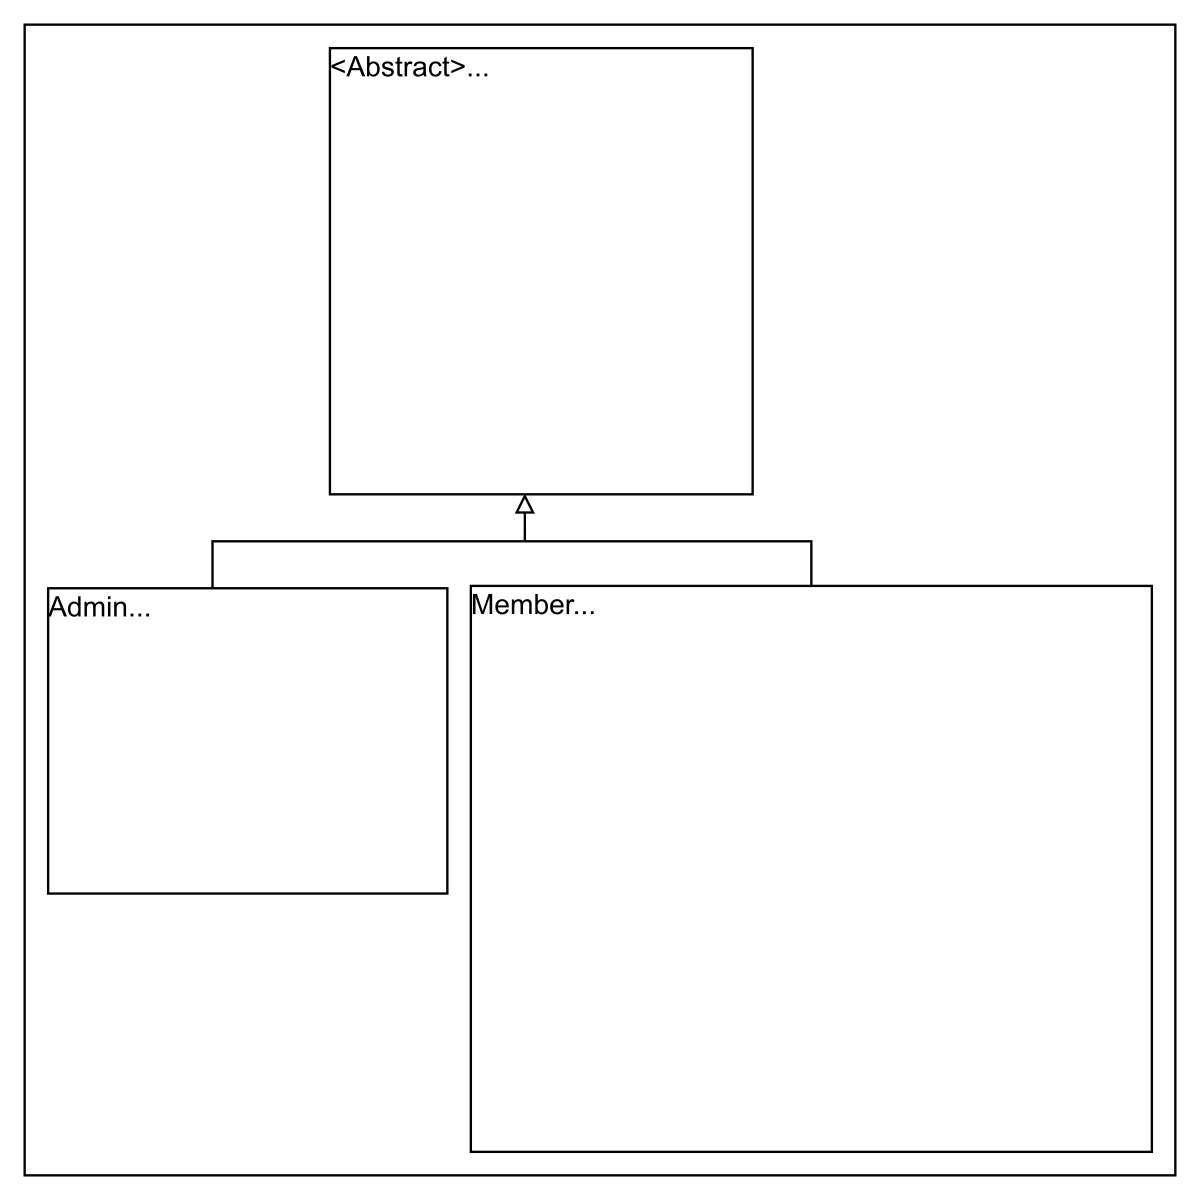
\includegraphics[width=0.5\textwidth]{Images/chapter_23/section_4575406147764224/5954868995817472.png}
 \caption{The class diagram of Account and its derived classes}
\end{figure}

\subsubsection{Watch list}\label{spPUwOm3kRzPiqkKehu98-2}
\\
A \textbf{watch list} is a list of stocks that an investor monitors to profit from price drops. Below is a visual representation of the \texttt{Watchlist} class.

\begin{figure}[htbp]
 \centering
 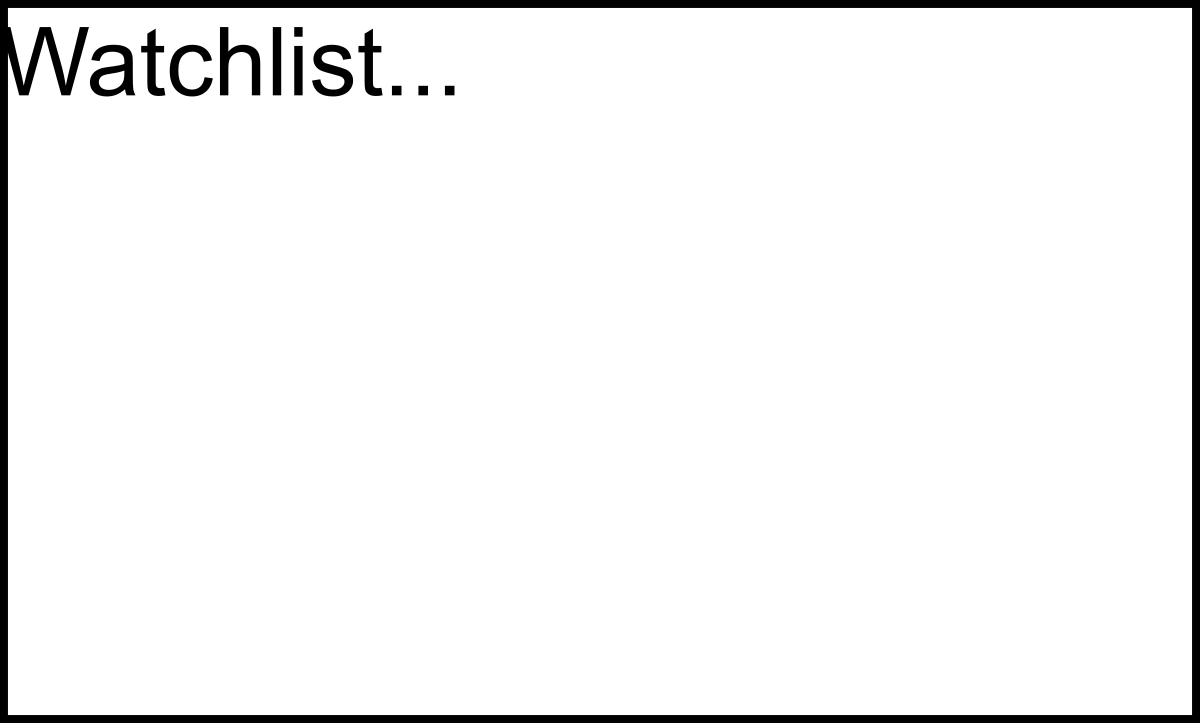
\includegraphics[width=0.5\textwidth]{Images/chapter_23/section_4575406147764224/5921698622996480.png}
 \caption{The class diagram of the Watchlist class}
\end{figure}

\textbf{R2:} Users can have numerous watch lists consisting of different stock quotes.

\subsubsection{Stock}\label{spPUwOm3kRzPiqkKehu98-3}
\\
A \textbf{stock}, also known as equity, is a security that represents a portion of the issuing company's ownership. The \texttt{Stock} class will have a symbol, price, etc.

\begin{figure}[htbp]
 \centering
 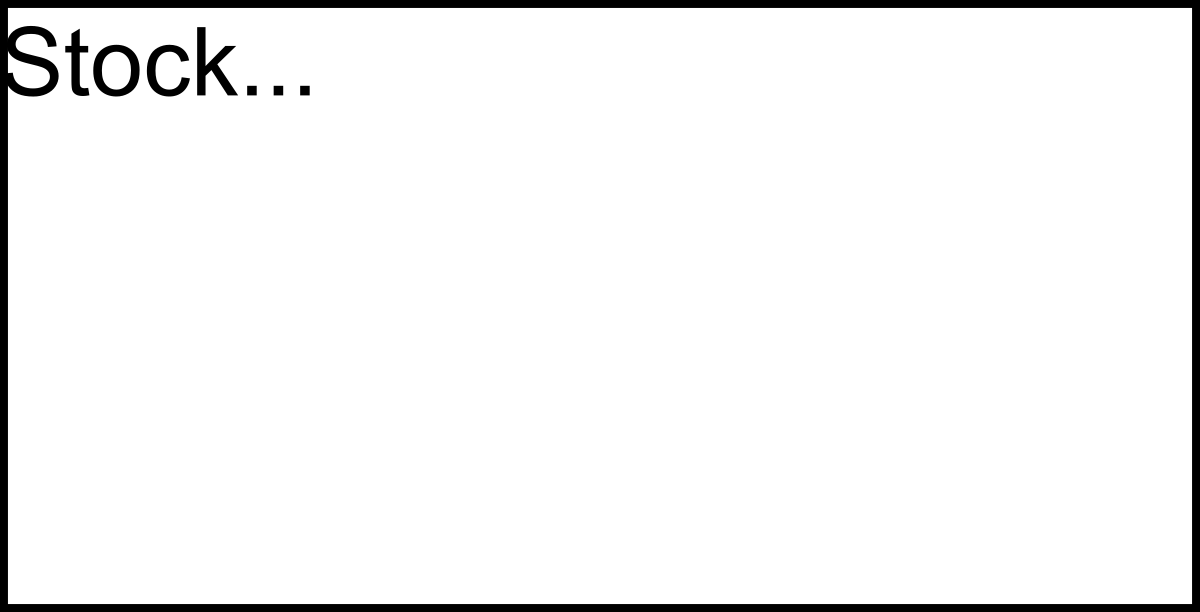
\includegraphics[width=0.5\textwidth]{Images/chapter_23/section_4575406147764224/6334917929861120.png}
 \caption{The class diagram of the Stock class}
\end{figure}

\textbf{R1:} The system should allow users to easily trade stocks (buy or sell them).

\subsubsection{Search and stock inventory}\label{spPUwOm3kRzPiqkKehu98-4}
\\
The \texttt{StockInventory} class will retrieve and keep up with the most recent stock values from the \texttt{StockExchange} class (defined later).~The \texttt{StockInventory} class implements the \texttt{Search} interface.

\begin{figure}[htbp]
 \centering
 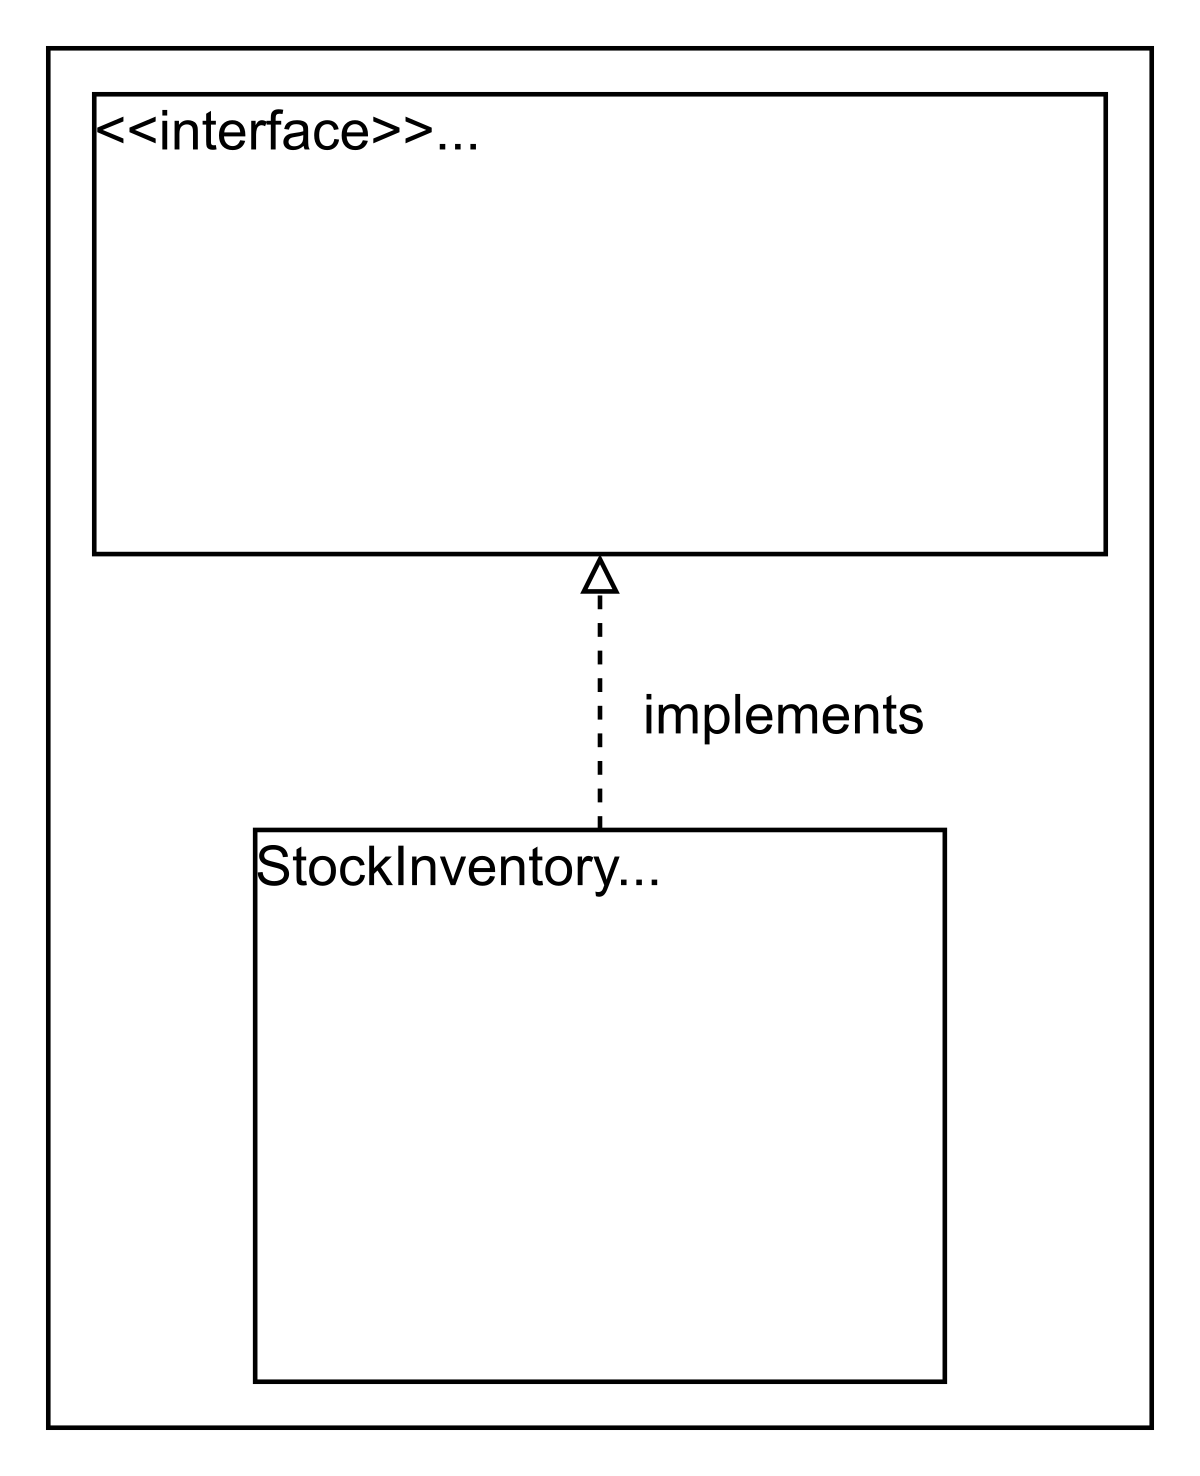
\includegraphics[width=0.5\textwidth]{Images/chapter_23/section_4575406147764224/5213401973129216.png}
 \caption{The class diagram of the Search interface and the StockInventory class}
\end{figure}

\subsubsection{Stock position}\label{spPUwOm3kRzPiqkKehu98-5}
\\
All the stocks the user owns will be included in the \texttt{StockPosition} class.

\begin{figure}[htbp]
 \centering
 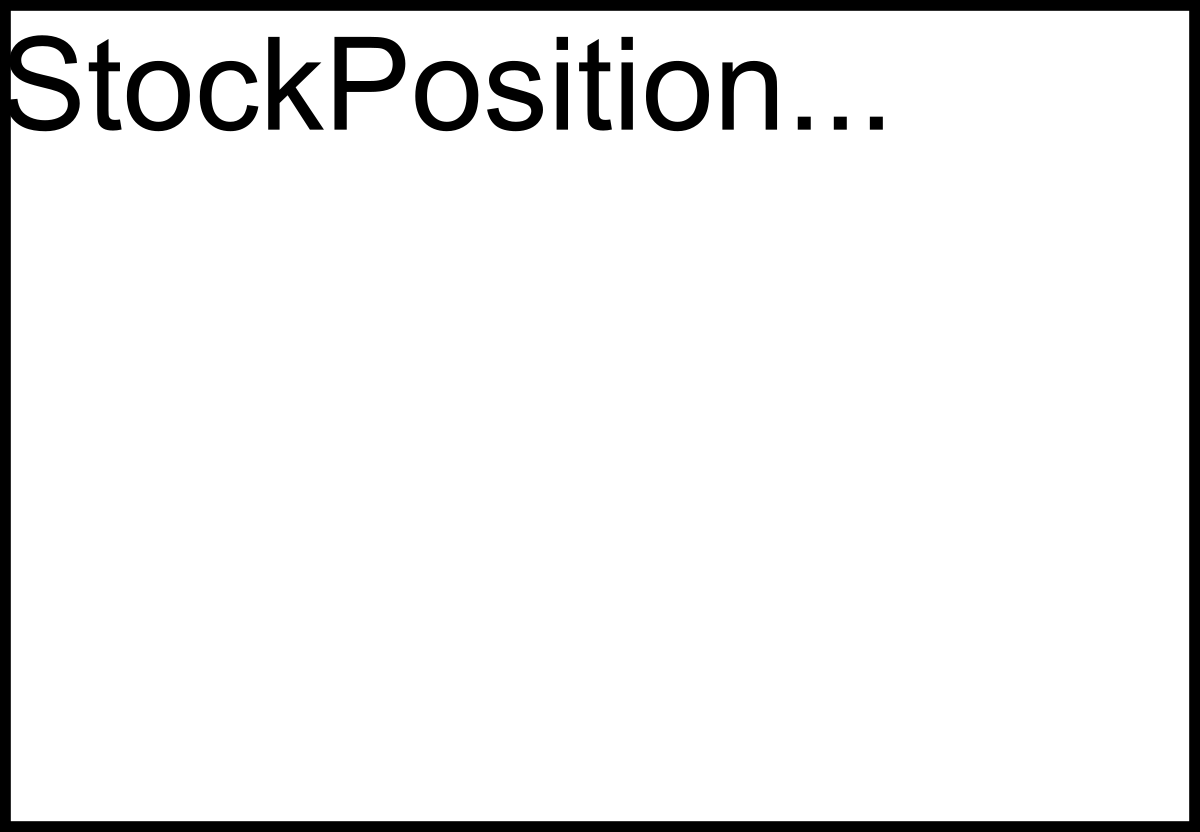
\includegraphics[width=0.5\textwidth]{Images/chapter_23/section_4575406147764224/6168571162132480.png}
 \caption{The class diagram of the StockPosition class}
\end{figure}

\subsubsection{Stock lot}\label{spPUwOm3kRzPiqkKehu98-6}
\\
A member may purchase various lots of the same stock on various dates. The \texttt{StockLot} class will represent these particular lots.

\begin{figure}[htbp]
 \centering
 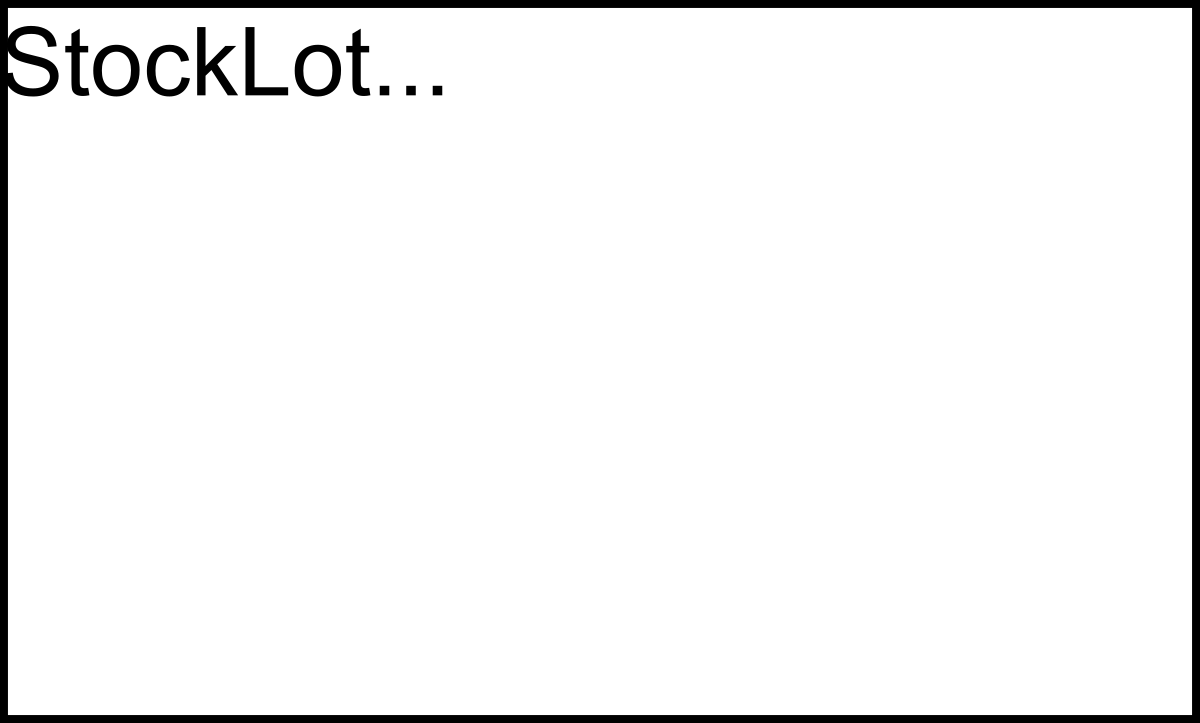
\includegraphics[width=0.5\textwidth]{Images/chapter_23/section_4575406147764224/5462031526526976.png}
 \caption{The class diagram of the StockLot class}
\end{figure}

\textbf{R3:} Users may own different lots of the same stock. If a user has purchased the same stock more than once, the system should be able to distinguish between several lots of it.

\subsubsection{Order}\label{spPUwOm3kRzPiqkKehu98-7}
\\
Members can place stock trading orders to sell or acquire stock positions. There are four types of orders supported by the system:
\\
\texttt{MarketOrder}\textbf{:} This allows customers to purchase or sell equities immediately at the market's going rate (current market price).
\\
\texttt{LimitOrder}\textbf{:} A user may specify a price at which they wish to purchase or sell a stock.
\\
\texttt{StopLossOrder}\textbf{:} An order to purchase or sell whenever the stock hits a specific price.
\\
\texttt{StopLimitOrder}\textbf{:} The \texttt{StopLimitOrder} becomes a limit order to purchase or sell at the limit price, or better, if the stop price is reached.

\begin{figure}[htbp]
 \centering
 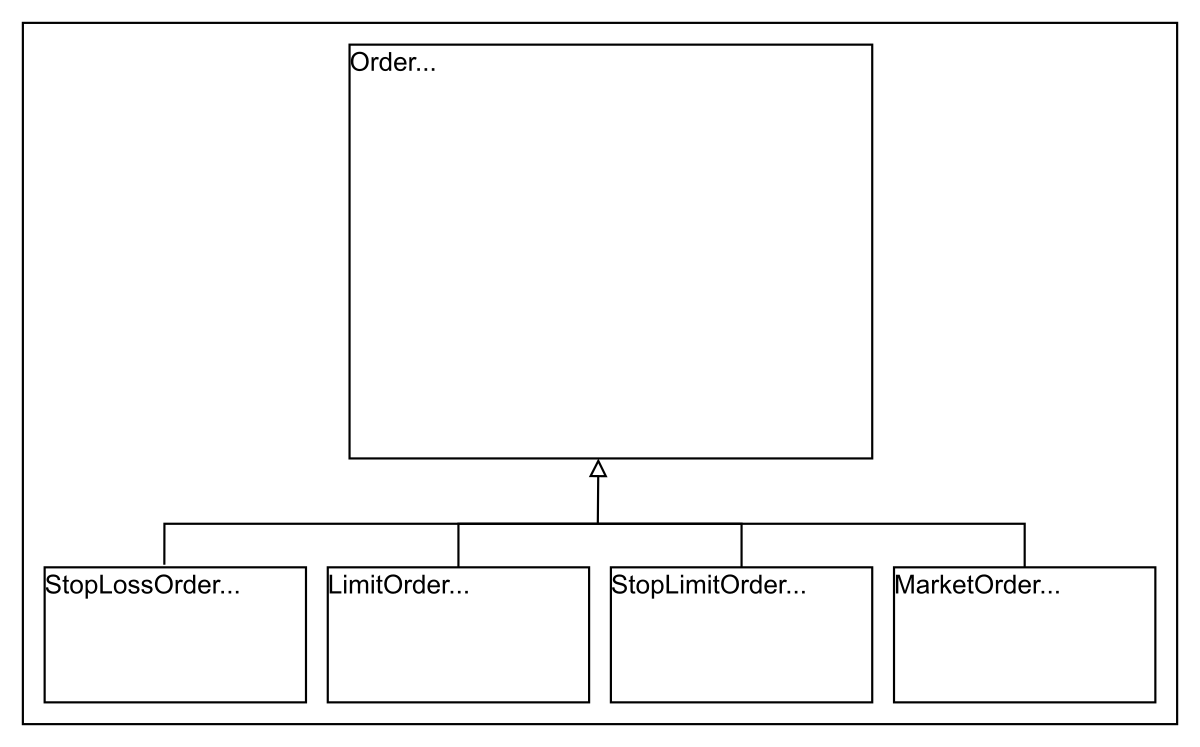
\includegraphics[width=0.5\textwidth]{Images/chapter_23/section_4575406147764224/4887098107494400.png}
 \caption{The class diagram of Order and its derived classes}
\end{figure}

\textbf{R5:} The system should allow the user to order the stock trade of the types given below:

\begin{itemize}
\tightlist
\item
\textbf{Market order:} Buy or sell stocks at the current market price.
\item
\textbf{Limit order:} Buy or sell stocks at the price set by the user.
\item
\textbf{Stop-loss order:} Buy or sell stocks when they reach a certain price.
\item
\textbf{Stop-limit order:} Buy or sell stocks with a restriction on the limit price (maximum price to be paid, minimum price to be received, etc).
\end{itemize}

\subsubsection{Order part}\label{AB3OHKqykpTu2fZ1e5qiw}
\\
Multiple order parts might be used to complete an order. The \texttt{OrderPart} class contains the price, quantity, and execution date.

\begin{figure}[htbp]
 \centering
 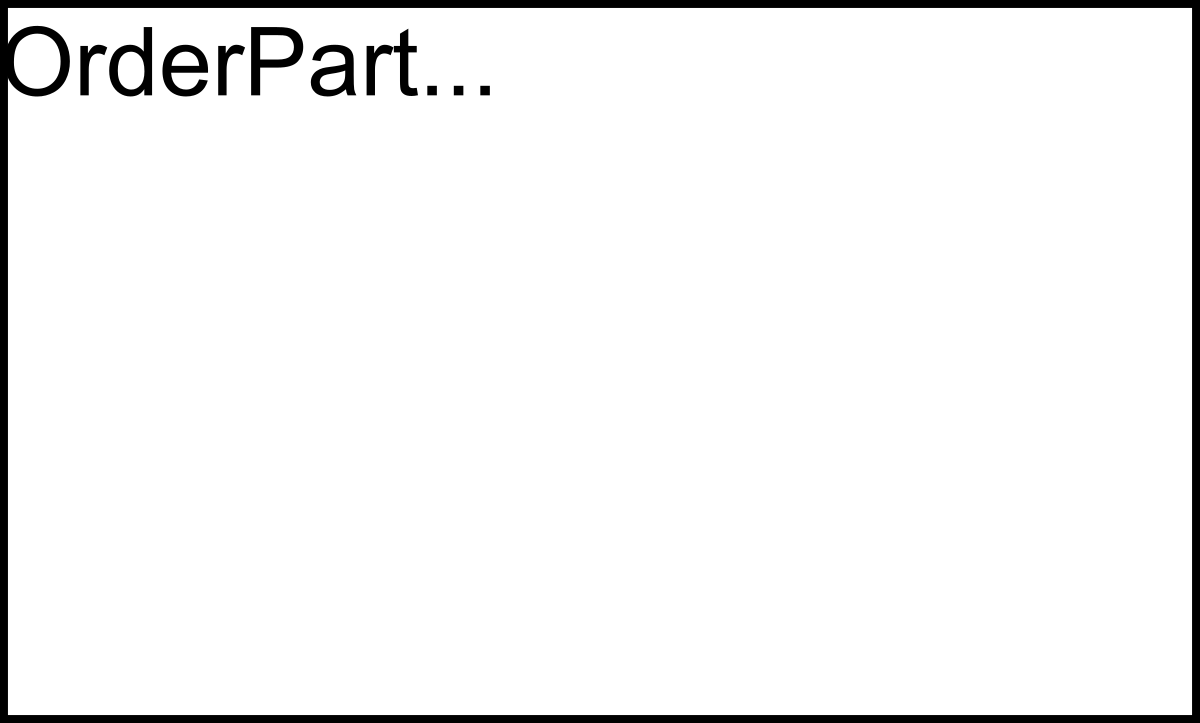
\includegraphics[width=0.5\textwidth]{Images/chapter_23/section_4575406147764224/6623468529647616.png}
 \caption{The class diagram of the OrderPart class}
\end{figure}

\subsubsection{Deposit and withdraw money}\label{spPUwOm3kRzPiqkKehu98-8}
\\
The \texttt{DepositMoney} class represents a transfer of money from one party to another.
\\
The \texttt{WithdrawMoney} class represents removing money from an account.

\begin{figure}[htbp]
 \centering
 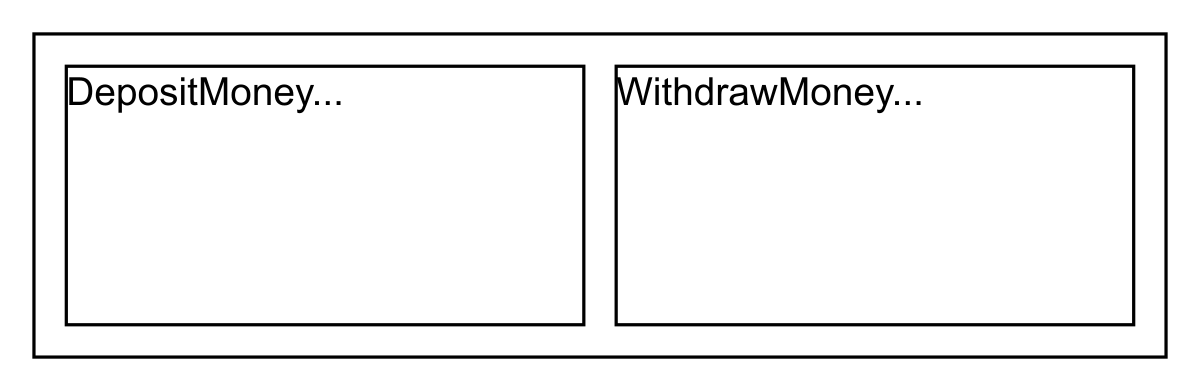
\includegraphics[width=0.5\textwidth]{Images/chapter_23/section_4575406147764224/5462933709389824.png}
 \caption{The class diagram of the DepositMoney and WithdrawMoney classes}
\end{figure}

\textbf{R6:} The system should allow users to make deposits and withdrawals using checks, wire transfers, or electronic bank transfers.

\subsubsection{Transfer money}\label{spPUwOm3kRzPiqkKehu98-9}
\\
Users should be able to deposit and withdraw money via check, wire, or electronic bank transfer.

\begin{figure}[htbp]
 \centering
 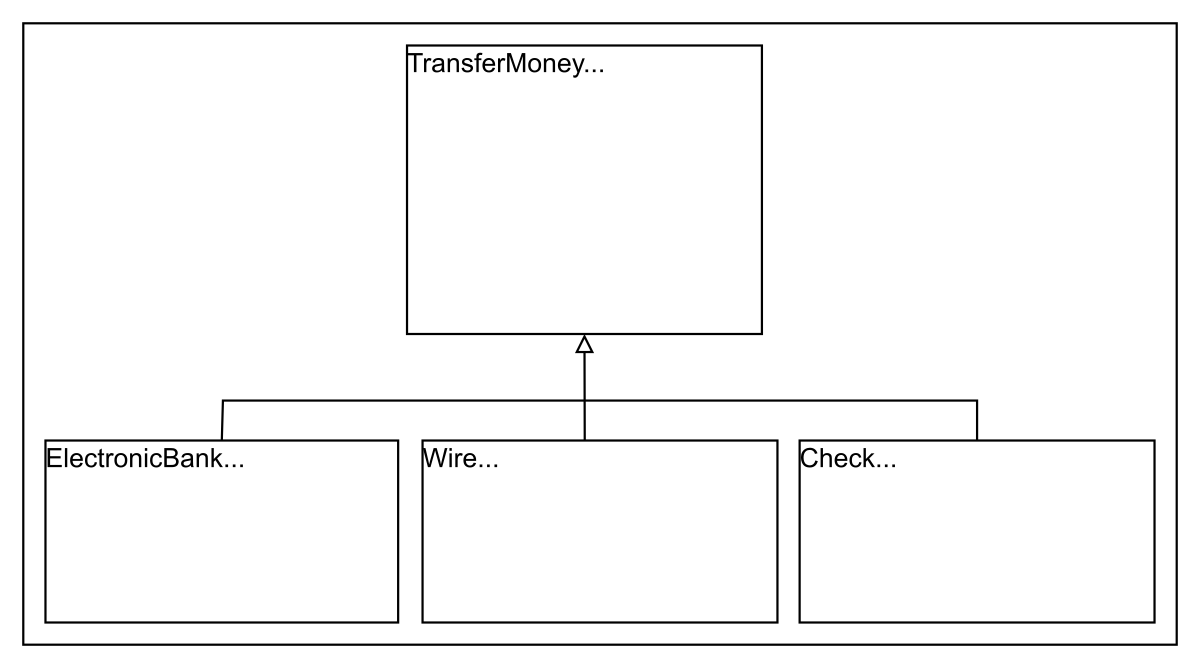
\includegraphics[width=0.5\textwidth]{Images/chapter_23/section_4575406147764224/6268654441070592.png}
 \caption{The class diagram of TransferMoney and its derived classes}
\end{figure}

\textbf{R6:} The system should allow users to make deposits and withdrawals using checks, wire transfers, or electronic bank transfers.

\subsubsection{Notification}\label{spPUwOm3kRzPiqkKehu98-10}
\\
\texttt{Notification} is an abstract class responsible for sending notifications when trade orders are executed. Every notification has an ID, creation date, and content. It can be an SMS or email notification.
\\
The\texttt{SmsNotification} class requires the member\textquotesingle s phone number to send a notification. The
\texttt{EmailNotification} class needs the member\textquotesingle s email address to send a notification. The relationship diagram of these classes is shown here:

\begin{figure}[htbp]
 \centering
 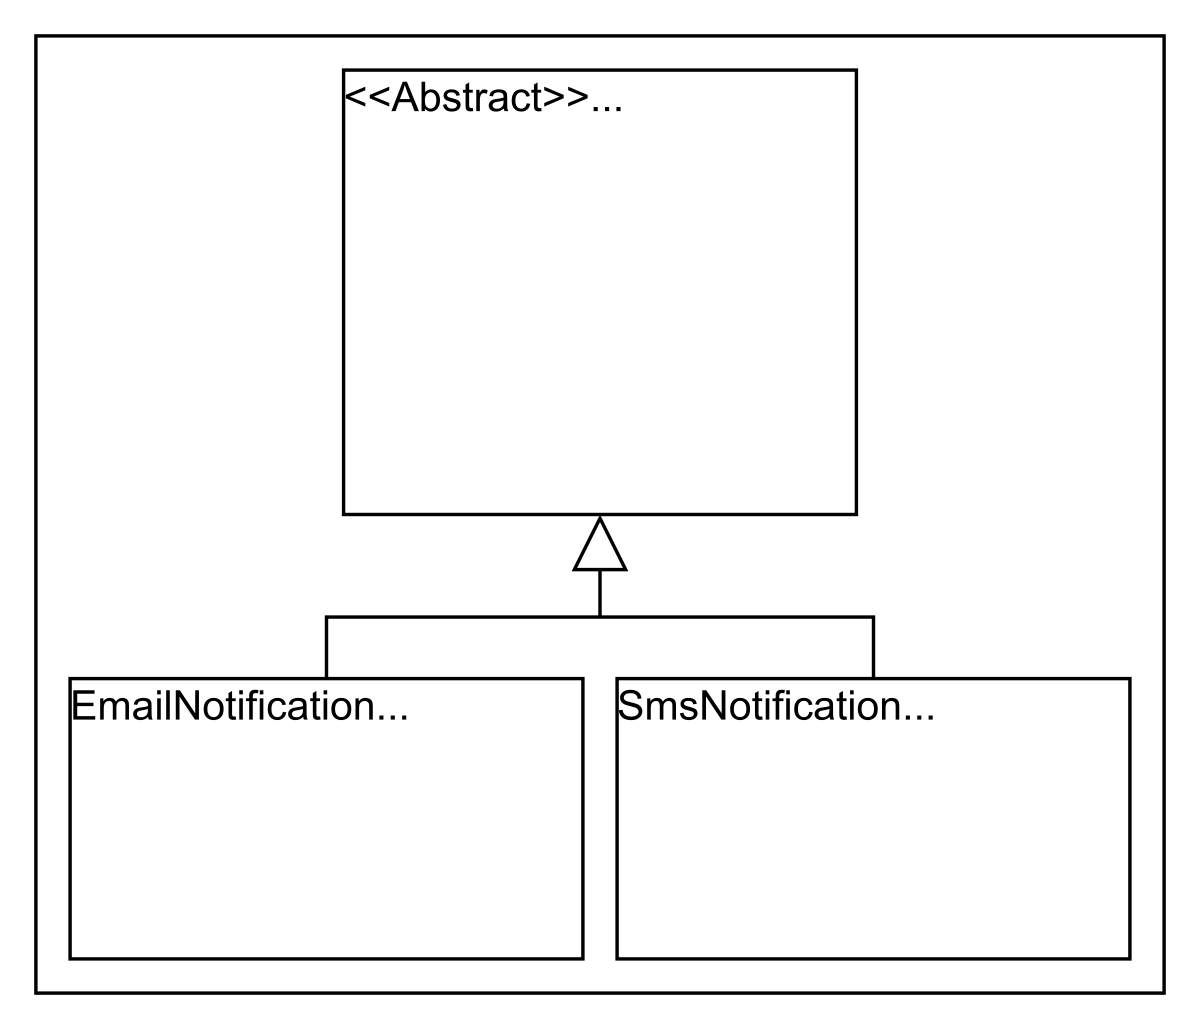
\includegraphics[width=0.5\textwidth]{Images/chapter_23/section_4575406147764224/6082424558452736.png}
 \caption{The class diagram of Notification and its derived classes}
\end{figure}

\textbf{R4:} The system should be able to notify users whenever a trade order is executed.

\subsubsection{Stock exchange}\label{spPUwOm3kRzPiqkKehu98-11}
\\
The stock brokerage system will get all stocks from the stock exchange and their current pricing. The
\texttt{StockExchange} class is responsible for creating orders for trading stocks on the stock exchange.

\begin{figure}[htbp]
 \centering
 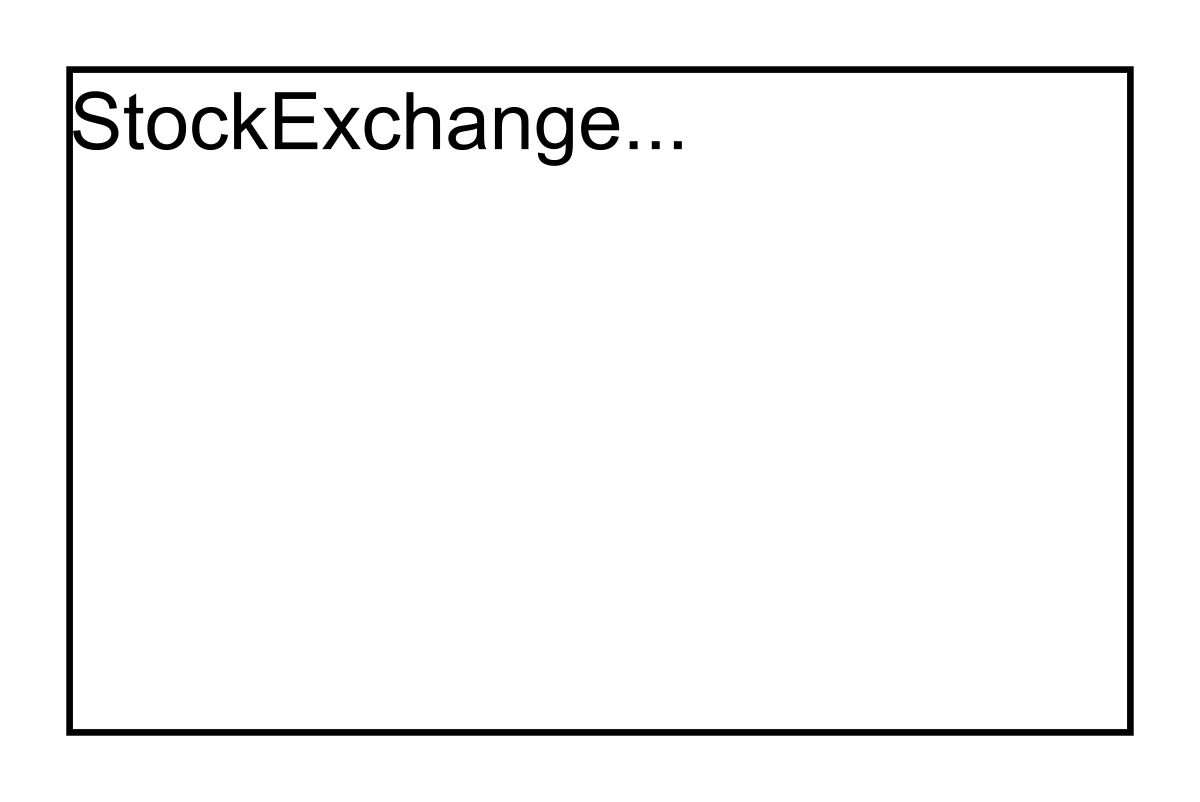
\includegraphics[width=0.5\textwidth]{Images/chapter_23/section_4575406147764224/4800461570703360.png}
 \caption{The class diagram of the StockExchange class}
\end{figure}

\subsubsection{Enumerations and custom data types}\label{spPUwOm3kRzPiqkKehu98-12}
\\
The following provides an overview of the enumerations and custom data types used in this problem:

\begin{itemize}
\item
\protect\phantomsection\label{lxET6YUftp3xdbiZXdiAl}
\texttt{OrderStatus}\textbf{:} We need to create an enumeration to keep track of the status of the order, whether it is open, filled\emph{,} partially filled, or canceled.
\end{itemize}

\begin{figure}[htbp]
 \centering
 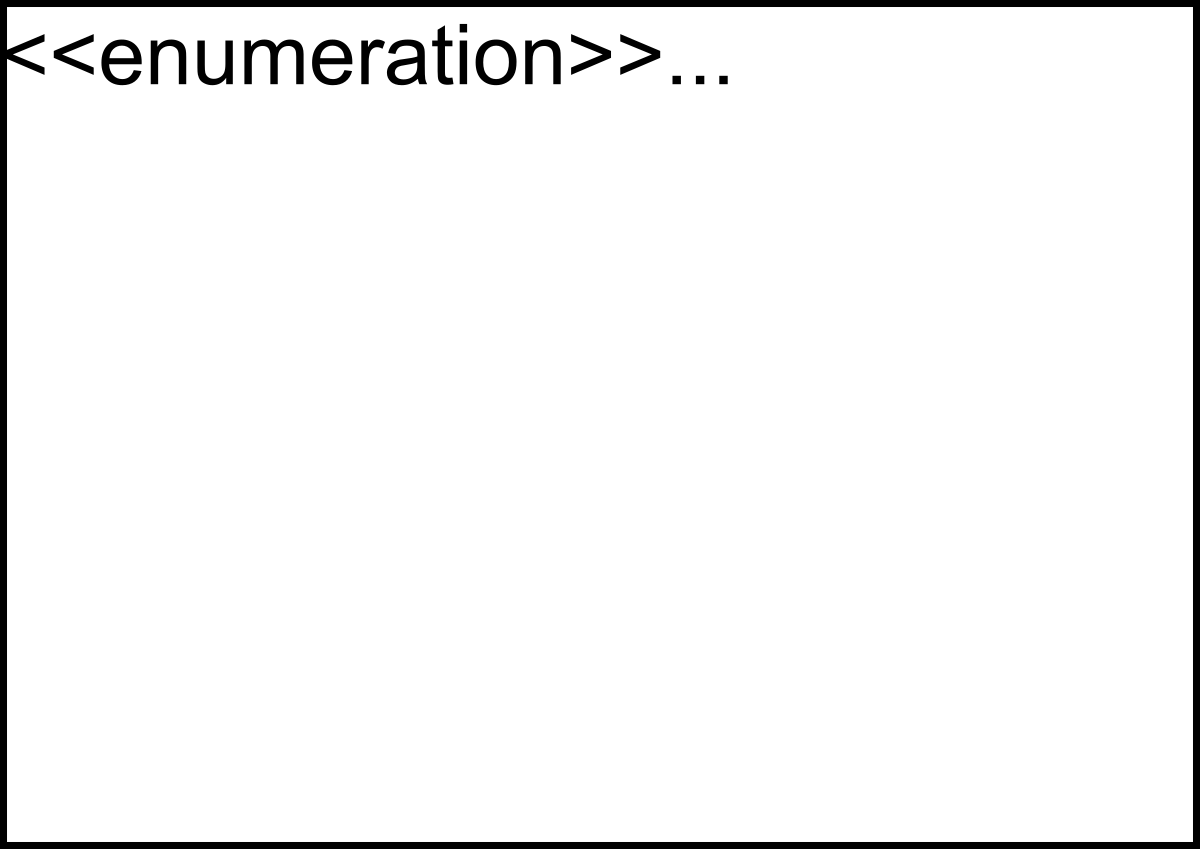
\includegraphics[width=0.5\textwidth]{Images/chapter_23/section_4575406147764224/5948614914605056.png}
 \caption{The OrderStatus enumerations}
\end{figure}

\begin{itemize}
\item
\protect\phantomsection\label{ETCqsnfV-fUJDYZEeOwFa}
\texttt{TimeEnforcementType}\textbf{:} We need to create an enumeration for the time enforcement type, whether it is good till canceled, fill or terminate, immediate or cancel, on the open, or on the close.
\end{itemize}

\begin{figure}[htbp]
 \centering
 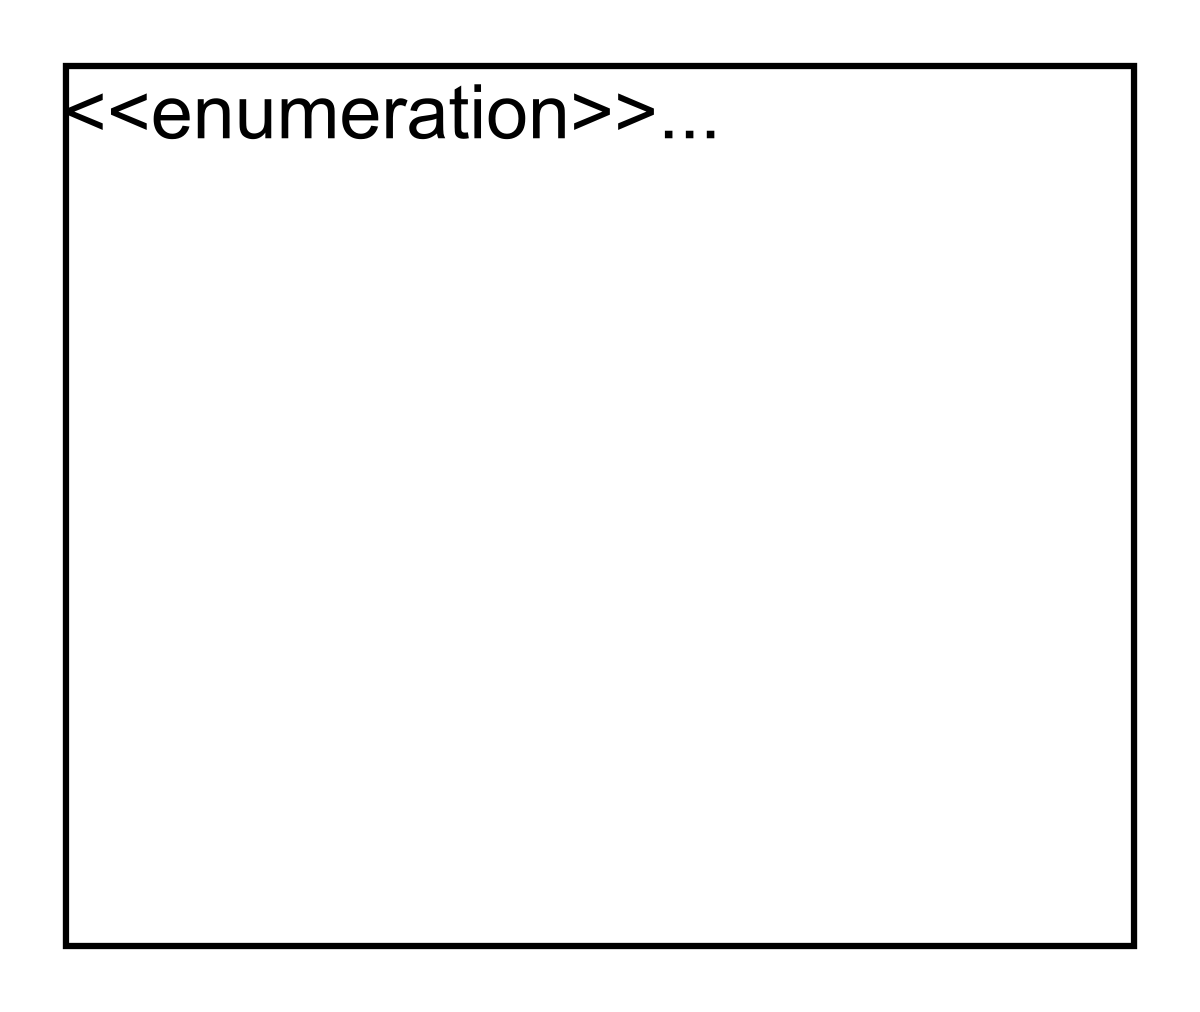
\includegraphics[width=0.5\textwidth]{Images/chapter_23/section_4575406147764224/6206018713157632.png}
 \caption{The TimeEnforcementType enumerations}
\end{figure}

\begin{itemize}
\item
\protect\phantomsection\label{6tOL4NpJomww0VepNzNdm}
\texttt{AccountStatus}\textbf{:} We need to create an enumeration to keep track of the account\textquotesingle s status, whether it is active, canceled, closed, blacklisted, or none.
\end{itemize}

\begin{figure}[htbp]
 \centering
 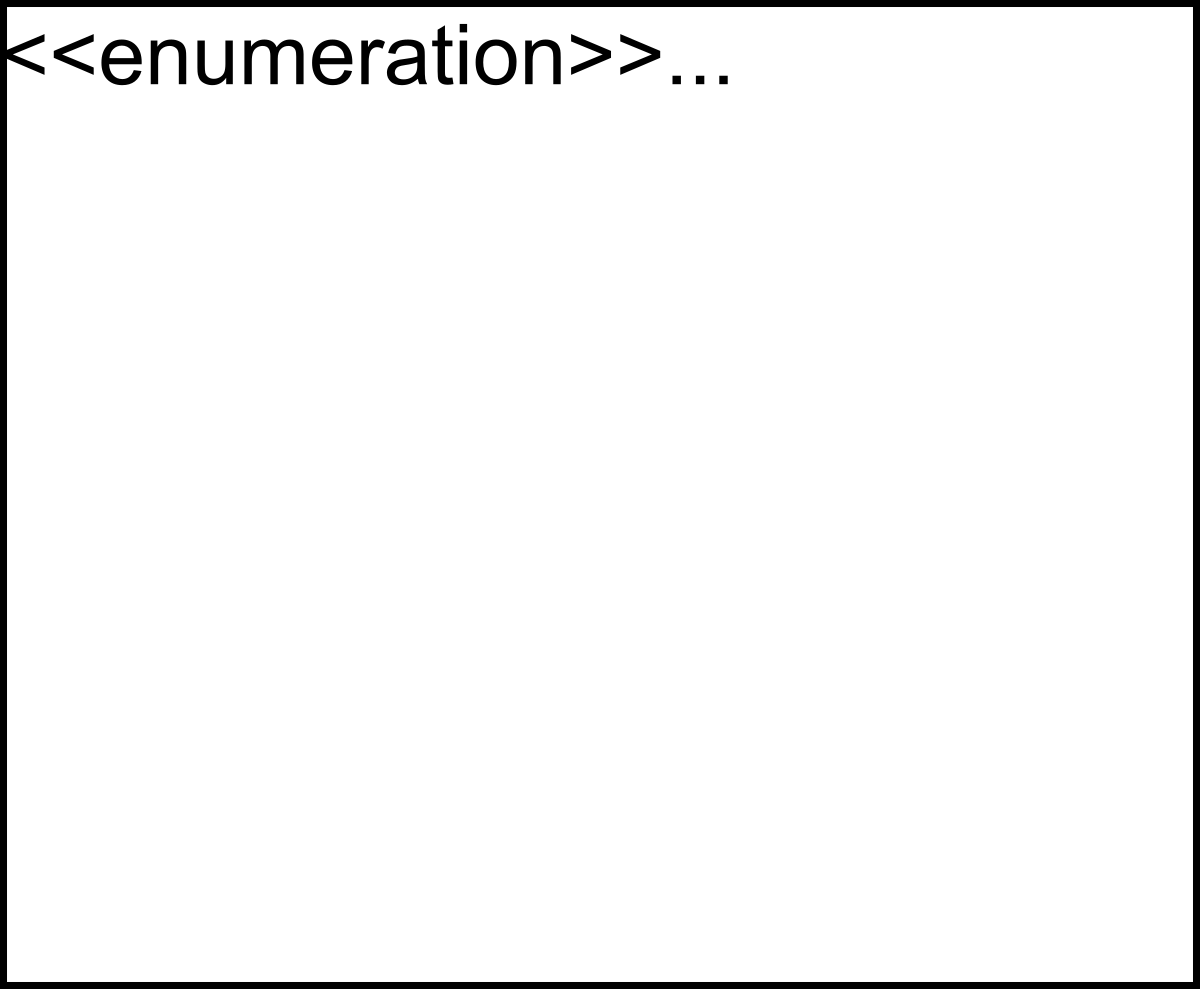
\includegraphics[width=0.5\textwidth]{Images/chapter_23/section_4575406147764224/6070382086062080.png}
 \caption{The AccountStatus enumerations}
\end{figure}

\begin{itemize}
\item
\protect\phantomsection\label{v3K3drhkbktSMO46ICysW}
\texttt{ErrorCode}\textbf{:} We need to create an enumeration to represent the outcome of operations, indicating whether they were successful, failed due to insufficient funds, invalid inputs, or were rejected for other reasons.
\end{itemize}

\begin{figure}[htbp]
 \centering
 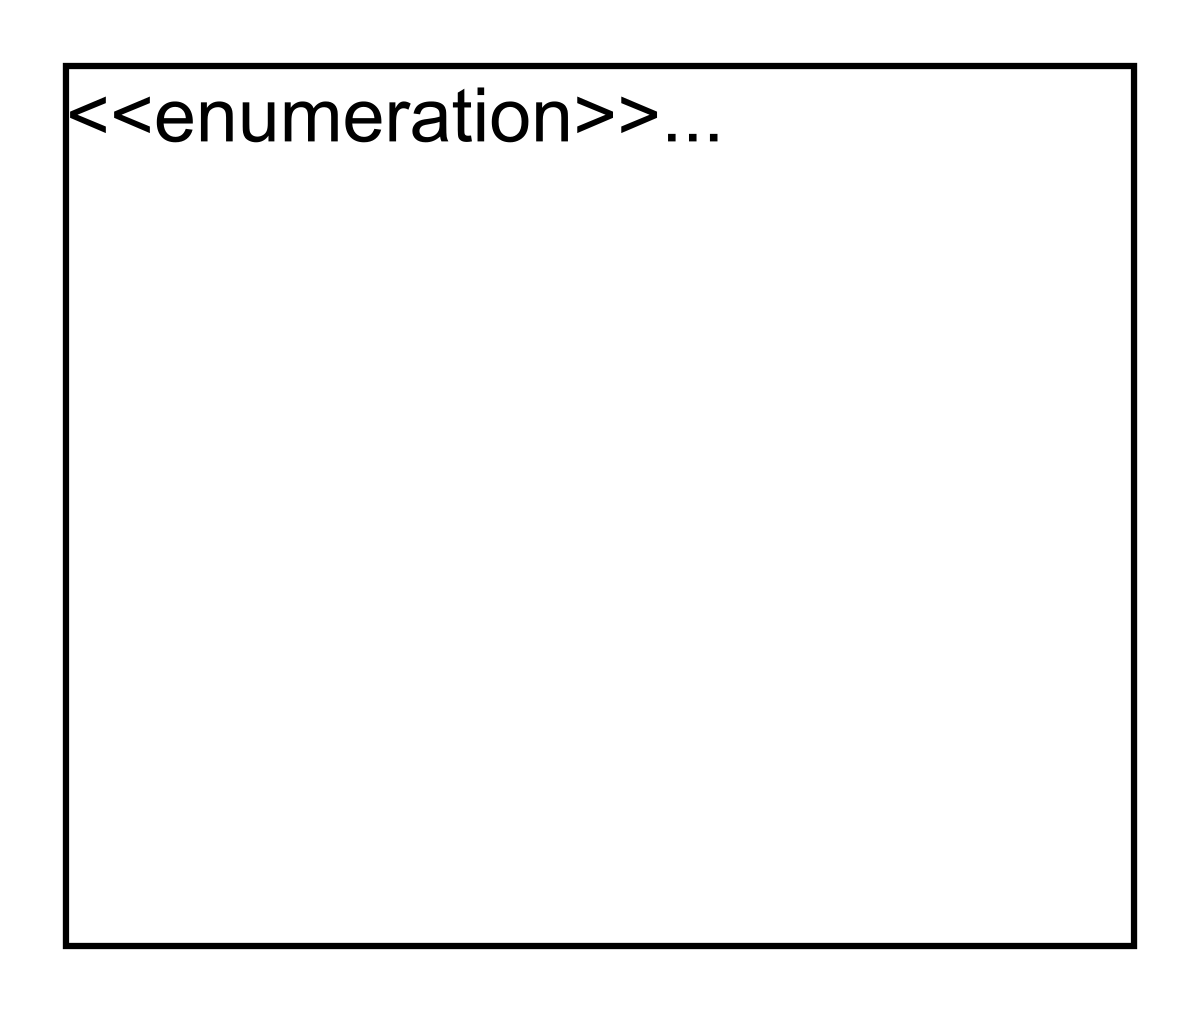
\includegraphics[width=0.5\textwidth]{Images/chapter_23/section_4575406147764224/6709855124324352.png}
 
\end{figure}

\paragraph{Address}\label{s0WnzmTN1ytDH9yWJ_rtS}
\\
We also need to create a custom data type, \texttt{Address}, to store the user\textquotesingle s location.

\begin{figure}[htbp]
 \centering
 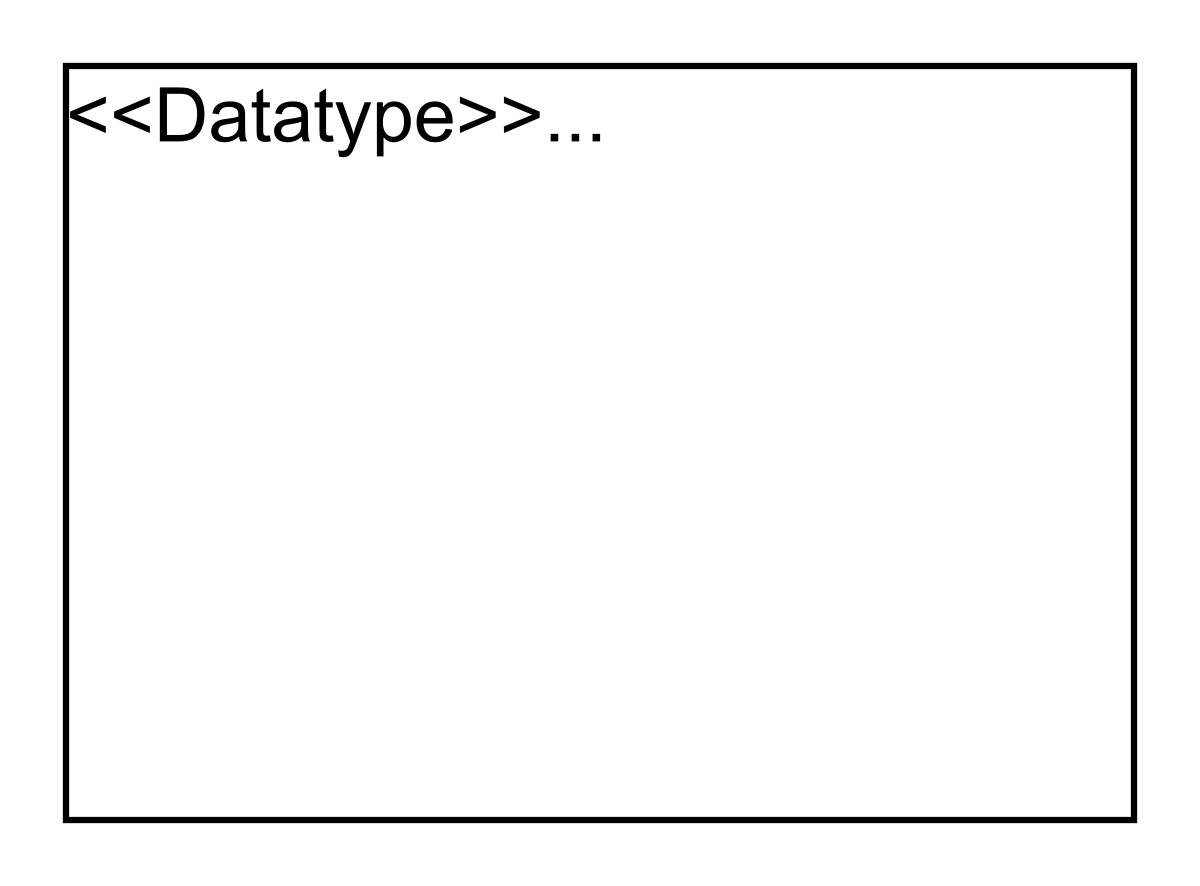
\includegraphics[width=0.5\textwidth]{Images/chapter_23/section_4575406147764224/6333178028359680.png}
 \caption{The class diagram of the Address class}
\end{figure}

\subsection{Relationship between the classes}\label{spPUwOm3kRzPiqkKehu98-13}
\\
Now, we'll discuss the relationships between the classes we have defined above in our online stock brokerage system.

\subsubsection{Association}\label{g4wjoPabmSB_pc1m4y17B}
\\
The class diagram has the following association relationships:
\\
\paragraph{One-way association}\label{38VkXUIpDvBS-VHQXNsSZ}

\begin{itemize}
\item
\protect\phantomsection\label{wIFFLVNbUcrUUMll-Euz0}
The \texttt{StockInventory} class has a one-way association with \texttt{Watchlist} and\texttt{StockExchange}.
\item
\protect\phantomsection\label{HPL73Lmj0JvsNb12rhAXB}
The \texttt{Order} class has a one-way association with \texttt{Stock}, \texttt{StockExchange}, and \texttt{StockLot}.
\item
\protect\phantomsection\label{Qo3SF_fPiQd-vFx1w2LzO}
The \texttt{Account} class has a one-way association with \texttt{Order}, \texttt{DepositMoney}\textbf{,} and\texttt{WithdrawMoney}\textbf{.}
\item
\protect\phantomsection\label{HWz9xTrLn-IOUIO7Dzlmt}
The \texttt{StockPosition} classhas a one-way association with the \texttt{Order} class.
\end{itemize}

\begin{figure}[htbp]
 \centering
 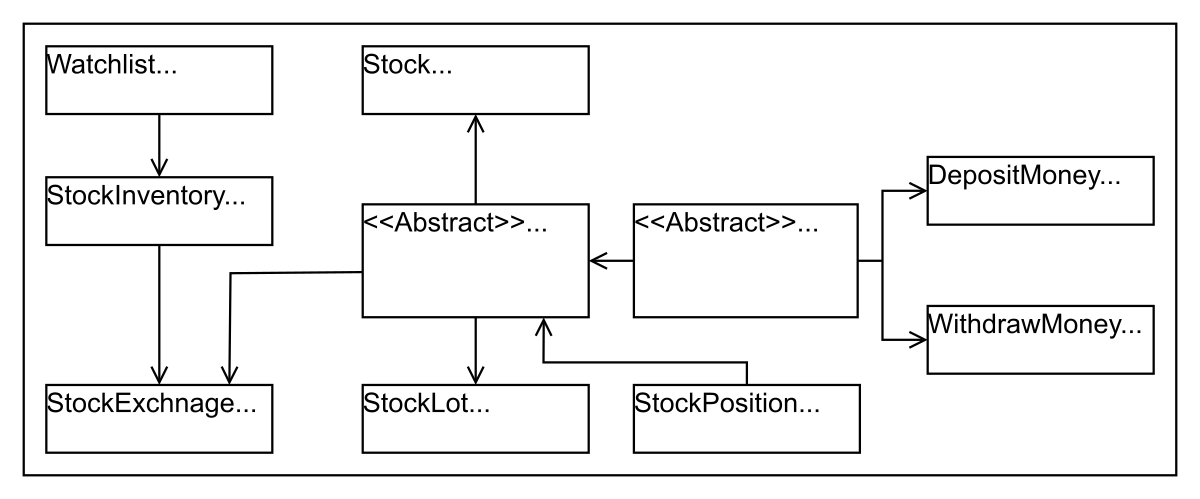
\includegraphics[width=0.5\textwidth]{Images/chapter_23/section_4575406147764224/6111051119460352.png}
 \caption{The one-way association relationship between classes}
\end{figure}

\paragraph{Two-way association}\label{A5aJabd4t9ShMc8TdNlWe}

\begin{itemize}
\item
\protect\phantomsection\label{qEpIT8ddNrBbTJldgM2Bh}
The \texttt{Notification} class has a two-way association with the \texttt{Order} class.
\item
\protect\phantomsection\label{PC8-xG0P0SgScajxexLJO}
Both \texttt{Watchlist} and\texttt{StockPosition} have a two-way association with the \texttt{Account} class.
\end{itemize}

\begin{figure}[htbp]
 \centering
 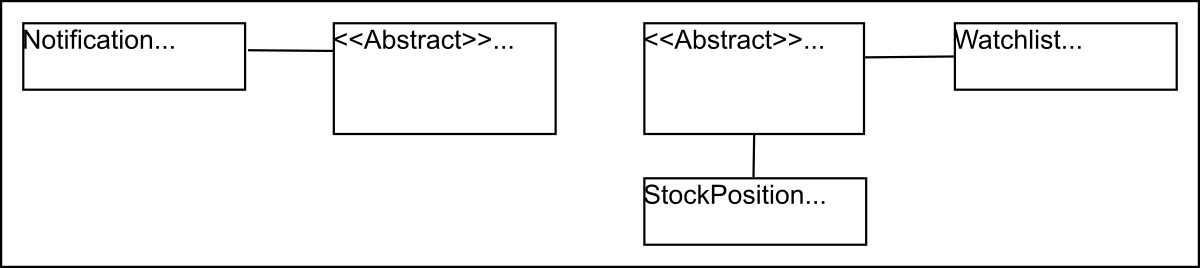
\includegraphics[width=0.5\textwidth]{Images/chapter_23/section_4575406147764224/5425978950287360.png}
 \caption{The two-way association relationship between classes}
\end{figure}

\subsubsection{Composition}\label{j9LKUkNT_QebF_q9mWfLi}
\\
The class diagram has the following composition relationships:

\begin{itemize}
\item
\protect\phantomsection\label{tyQHGJ7d0aBoVCgbSkonk}
The \texttt{Order} classis composed of \texttt{OrderPart}.
\item
\protect\phantomsection\label{JCD36Z1lCgNF1WsAJ5t_4}
The \texttt{StockInventory} class is composed of \texttt{Stock}.
\item
\protect\phantomsection\label{qUr5_g5q3iNjrPG3OnV87}
The \texttt{StockPosition} class is composed of \texttt{StockLot}.
\end{itemize}

\begin{figure}[htbp]
 \centering
 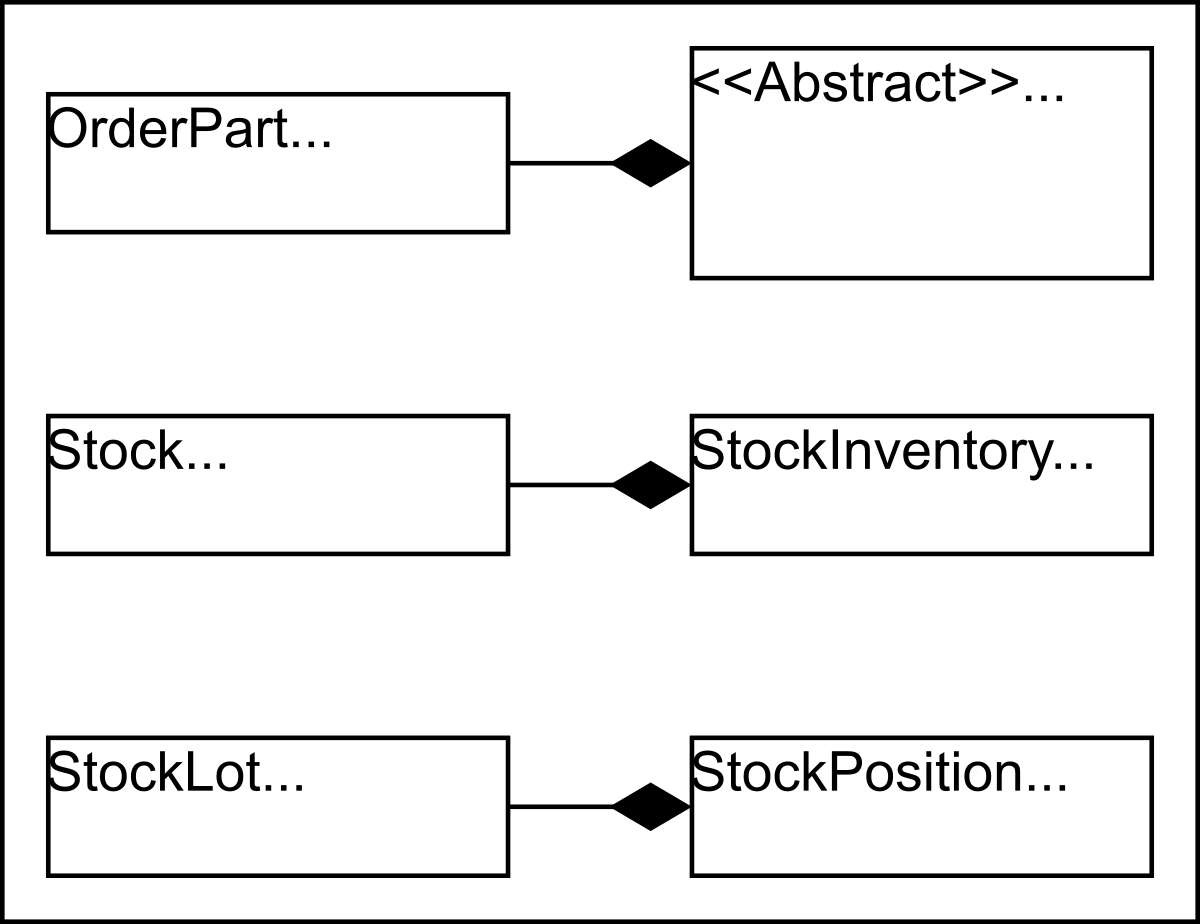
\includegraphics[width=0.5\textwidth]{Images/chapter_23/section_4575406147764224/5700906987552768.png}
 \caption{The composition relationship between classes}
\end{figure}

\subsubsection{Inheritance}\label{VB-a0gzbl1Vlz8sozqCrS}
\\
The following classes show an inheritance relationship:

\begin{itemize}
\item
\protect\phantomsection\label{AahJrwn5lh6ZZGK_xoSVg}
Both \texttt{Admin} and \texttt{Member} extend the \texttt{Account} class.
\item
\protect\phantomsection\label{TGJmhysIuIrq-J3UxTsvz}
The \texttt{MarketOrder}, \texttt{LimitOrder}, \texttt{StopLimitOrder}, and \texttt{StopLossOrder} classes extend the \texttt{Order} class.
\item
\protect\phantomsection\label{YS4wQsVQcfh9to-iTtQ6t}
The \texttt{ElectronicBank}, \texttt{Wire}, and \texttt{Check} classes extend the \texttt{TransferMoney} class.
\item
\protect\phantomsection\label{EhlOYoSBDuPRiBjVzWIPx}
The \texttt{SmsNotification} and \texttt{EmailNotification} classes extend the \texttt{Notification} class.
\item
\protect\phantomsection\label{-p9hY1vINCtxh8IvW9cZL}
The \texttt{StockInventory} class implements the \texttt{Search} interface.
\end{itemize}
\begin{quote}
\textbf{Note:} We have already discussed the inheritance relationship between classes in the component section above one by one.
\end{quote}
\subsection{Class diagram of the online stock brokerage system}\label{bJQQQJ-QQApU6H2WxM6xd}
\\
This section outlines the multiplicity (cardinality) relationships between the main classes in our online stock brokerage system. We explain the allowed number of instances on each side for each relationship and the real-world or design rationale behind the connection. Understanding these relationships is key to modeling how different entities interact and collaborate to support key workflows in the system.

\begin{table}[h!]
\centering
\begin{tabularx}{\textwidth}{|X|X|X|X|}
\hline
\textbf{Source} & \textbf{Target} & \textbf{Multiplicity} & \textbf{Description} \\
\hline
StockExchange & Order & 1 – 0..* & A stock exchange can receive multiple orders. \\
\hline
StockExchange & OrderPart & 1 – 0..* & A stock exchange manages multiple order parts. \\
\hline
Watchlist & Stock & 0..* & A watchlist can contain multiple stocks. \\
\hline
StockInventory & Stock & 1 – 0..* & Inventory may manage multiple stocks. \\
\hline
Order & OrderPart & 1 – 0..* & An order is composed of multiple order parts. \\
\hline
Notification & EmailNotification & 0..* & Generalization/Inheritance. \\
\hline
Notification & SmsNotification & 0..* & Generalization/Inheritance. \\
\hline
Account & Address & 1 – 1 & Each account has one address. \\
\hline
Account & DepositMoney & 1 – 0..* & An account can have multiple deposit transactions. \\
\hline
Account & WithdrawMoney & 1 – 0..* & An account can have multiple withdrawal transactions. \\
\hline
Admin & Account & 1 – 1 & Admin inherits from Account. \\
\hline
Member & Account & 1 – 1 & Member inherits from Account. \\
\hline
Member & StockPosition & 1 – 0..* & A member may hold multiple stock positions. \\
\hline
Member & Order & 1 – 0..* & A member can place multiple orders. \\
\hline
StockPosition & Stock & 1 – 1 & A stock position is related to one stock. \\
\hline
TransferMoney & ElectronicBank & 1 – 1 & Transfer via electronic bank. \\
\hline
TransferMoney & Wire & 1 – 1 & Transfer via wire. \\
\hline
TransferMoney & Check & 1 – 1 & Transfer via check. \\
\hline
StopLossOrder & Order & 1 – 1 & StopLossOrder inherits from Order. \\
\hline
LimitOrder & Order & 1 – 1 & LimitOrder inherits from Order. \\
\hline
StopLimitOrder & Order & 1 – 1 & StopLimitOrder inherits from Order. \\
\hline
MarketOrder & Order & 1 – 1 & MarketOrder inherits from Order. \\
\hline
StockLot & Order & 1 – 1 & Each stock lot is linked to one buying order. \\
\hline
\end{tabularx}
\caption{Stock Exchange System Entity Relationships}
\label{tab:stock_exchange_relationships}
\end{table}

Here is the complete class diagram for our online stock brokerage system:

\begin{figure}[htbp]
 \centering
 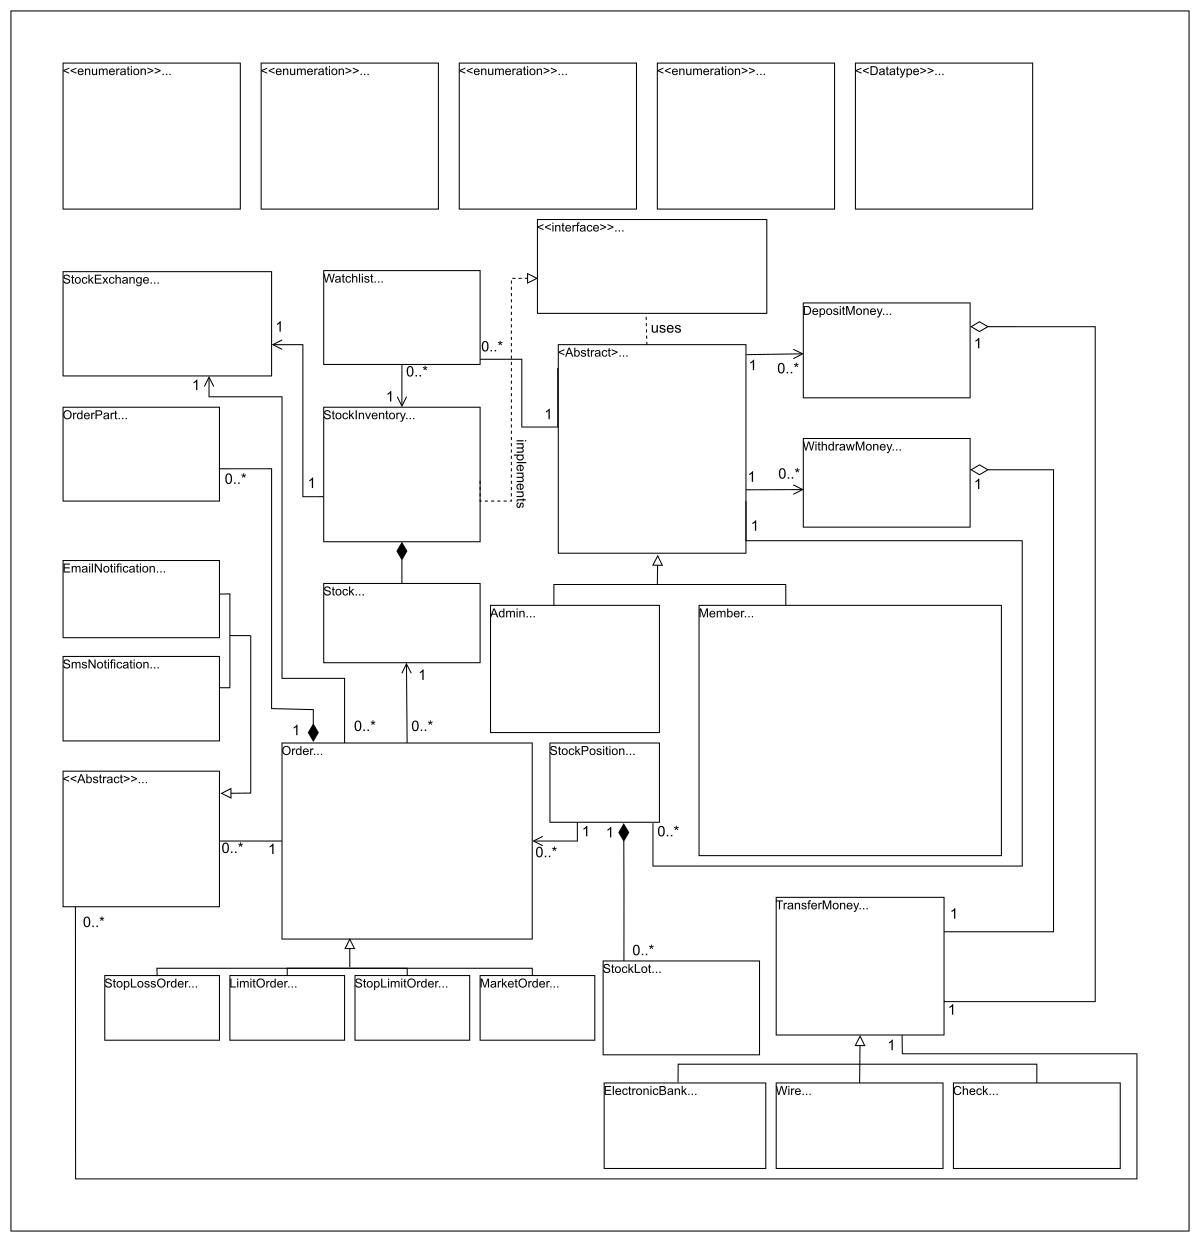
\includegraphics[width=0.5\textwidth]{Images/chapter_23/section_4575406147764224/4680814933442560.png}
 \caption{The class diagram of the online stock brokerage system}
\end{figure}

\subsection{Design pattern}\label{LvjigOzOcGZdSo4_6YDzQ}
\\
To implement online stock brokerage's core features in a flexible and scalable way, we apply the object-oriented design patterns based on system behavior.

\begin{itemize}
\item
The trading system handles different types of orders, such as market, limit, stop-loss, and stop-limit. We can use the Factory design pattern to manage the creation of these order types efficiently.
\item
The system processes payments through multiple channels, such as electronic bank, wire, or check. The Strategy design pattern can encapsulate these varying payment methods.
\item
Users or watch lists may want to be notified when a stock's price changes. W\textbackslash sout\{e\} can use the Observer design pattern to model this real-time notification behavior.
\item
Notifications can be sent via different channels, like email or SMS, and we might want to extend this with extra features like logging. To support this extensibility, we can use the Decorator design pattern.
\item
We know that only one \texttt{StockExchange} instance should be shared across the application. To ensure this, we can use the Singleton design pattern.
\item
We know that the process of sending a notification may follow a common structure but differ in implementation (email vs. SMS). We can use the Template Method design pattern to enforce this structure while allowing customization.
\item
We know that placing an order or sending a notification may need to be queued, logged, or executed later. We can use the Command design pattern to encapsulate these requests as objects.
\item
We know an order may consist of multiple parts, each with its own quantity and price, but we want to treat them as a single entity. To achieve this, we can use the Composite design pattern.
\item
Creating a complex order with multiple parts, statuses, and configurations can involve many steps. We can use the Builder design pattern to simplify and organize this process.
\end{itemize}

\subsection{AI-powered trainer}\label{Wzdqy9usDCKMRJ1y2PNyD}
\\
At this stage, everything should be clear. If you encounter any confusion or ambiguity, feel free to utilize the interactive AI-enabled widget below to seek clarification. This tool is designed to help you strengthen your understanding of the concepts.

\begin{figure}[htbp]
 \centering
 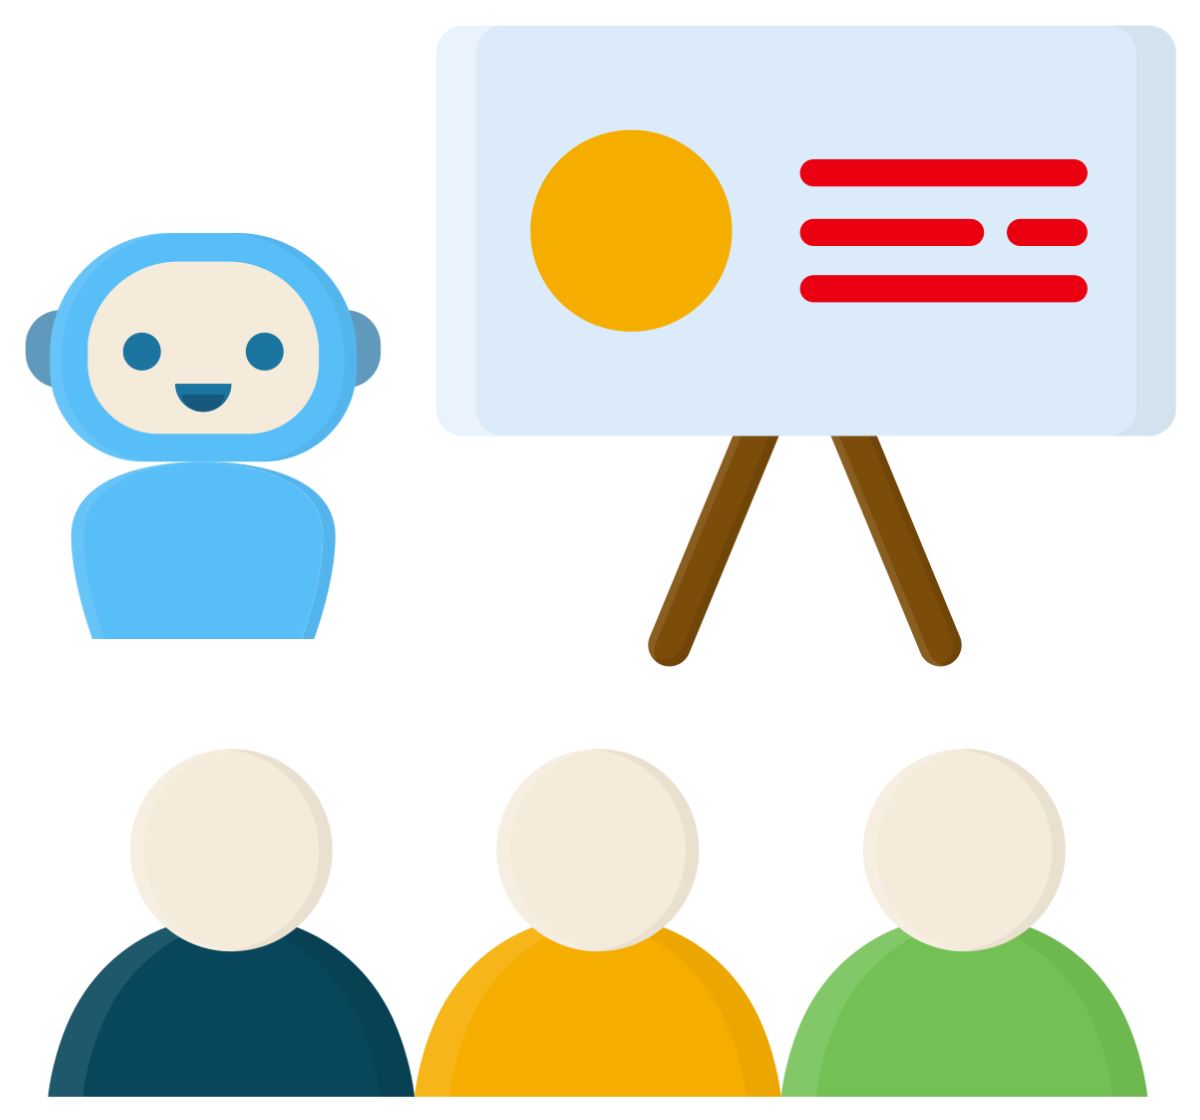
\includegraphics[width=0.15\textwidth]{Images/chapter_23/section_4575406147764224/6152612112891904.png}
 
\end{figure}

\textit{Component type 'PromptAI' not yet supported.}

We have successfully designed the class diagram for the online stock brokerage system. Let 's move to the next lesson to see how we can construct the sequence diagram for the system.

% End of section content